\chapter[TrES-4: A Transiting Hot Jupiter of Very-Low Density]%
{%
TrES-4: A Transiting Hot Jupiter of Very-Low Density%
\protect\CFNG%
}
\label{cha:tres4}

\section*{Abstract}
\label{cha:tres4:sec:abs}
\addcontentsline{toc}{section}{Abstract}

We report the discovery of \tresFour, a hot Jupiter that transits the star GSC 02620-00648 every 3.55\,days. From high-resolution spectroscopy of the star 
we estimate a stellar effective temperature of \mbox{$T_{\rm eff} = 6100 \pm 150$\,K}, 
and from high-precision $z$ and $B$ photometry of the transit we constrain the 
ratio of the semi-major axis $a$ and the stellar radius $R_{\star}$ to be 
\mbox{$a/R_{\star} = 6.03 \pm 0.13$}. We compare these values to model stellar 
isochrones to constrain the stellar mass to be 
\mbox{$M_{\star} = 1.22 \pm 0.17$\,$M_{\sun}$}. Based on this estimate and the photometric time series, we constrain the stellar radius to be 
\mbox{$R_{\star} = 1.738 \pm 0.092$\,$R_{\sun}$} and the planet radius to be 
\mbox{$R_{\rm p} = 1.674 \pm 0.094$\,$R_{\rm Jup}$}. We model our radial-velocity data assuming a circular orbit and find a planetary mass of 
$0.84 \pm 0.10$\,$M_{\rm Jup}$. Our radial-velocity observations rule out 
line-bisector variations that would indicate a specious detection resulting 
from a blend of an eclipsing binary system. \tresFour\ has the largest radius and 
lowest density of any of the known transiting planets. It presents a challenge 
to current models of the physical structure of hot Jupiters, and indicates that 
the diversity of physical properties among the members of this class of 
exoplanets has yet to be fully explored.

\section{Understanding the Mass--Radius Relations of Exoplanets}
\label{cha:tres4:sec:intro}

Despite the ever increasing number of discovered transiting planets (19 at the 
time of writing), our understanding of the relationships between host star 
properties and the planets' physical and orbital parameters is still 
incomplete. 
While the mass-radius relation 
for most transiting planets agrees with the models \citep{Charbonneau_Brown_Burrows:PPV:2007a}, several 
planets have either too high or too low densities. In particular, HD209458b 
\citep{Knutson_Charbonneau_Noyes:apj:2007a}, HAT-P-1b \citep{Bakos_Noyes_Kovacs:apj:2007a}, and WASP-1b \citep{Collier-Cameron_Bouchy_Hebrard:MNRAS:2007a} all have 
much larger radii and lower densities than expected for planets of their 
mass and distance from the host star. Several mechanisms for explaining this 
discrepancy have been proposed, among them different internal heat sources 
(\citealp{Guillot_Showman:aa:2002a}, \citealp*{Bodenheimer_Laughlin_Lin:apj:2003a}), increased planetary atmospheric opacities 
\citep{Burrows_Hubeny_Budaj:apj:2007a}, and less efficient heat transport as a result of interior composition gradient (Chabrier \& Baraffe \citeyear{Chabrier_Baraffe:apjl:2007a}). 
Our Trans-atlantic Exoplanet Survey (TrES) has previously announced the 
discovery of three transiting planets (Alonso et al., \citeyear{Alonso_Brown_Torres:apjl:2004a};  O'Donovan et al., \citeyear{ODonovan_Charbonneau_Mandushev:apjl:2006a}, see chapter~\ref{cha:tres2}; \citealp{ODonovan_Charbonneau_Bakos:apjl:2007a}, see chapter~\ref{cha:tres3}), each with distinctive properties. We describe here the newly discovered transiting planet \tresFour, whose mean density of $\rho = 0.222 \pm 0.045$~${\rm g \: cm^{-3}}$ is the lowest of all known exoplanets with measured radii and masses. 

\section{Photometry and Spectroscopy of \tresFour}
\label{cha:tres4:sec:obs}

We monitored a $5\fdg8 \times 5\fdg8$ field in Hercules with the Lowell 
Observatory Planet Search Survey Telescope \citep[PSST, ][]{Dunham_Mandushev_Taylor:pasp:2004a} and the 
Sleuth telescope \citep{ODonovan_Charbonneau_Kotredes:AIP:2004a} at Palomar Observatory between UT 2006 May~6 and 2006 August~2. 
All images were 
processed and the photometry and transit search carried out as described in 
\citet{Dunham_Mandushev_Taylor:pasp:2004a}. 
Both telescopes detected transits of the host star 
GSC~02620-00648: PSST observed 2 full and 1 partial transits, and Sleuth 
observed 3 full and 4 partial transits. The shape of the events 
were consistent with the transit of a Jupiter-sized planet across an F dwarf, 
and we undertook a program of follow-up observations to confirm the planetary 
nature of the object.

\begin{deluxetable}{llcc}
\tablewidth{0pt}
\tablecaption{\tresFour\ host star \label{cha:tres4:sec:obs:tab:host_star}}
\tablehead{
\colhead{Parameter} & \colhead{Units} & \colhead{Value} & \colhead{Source}}
\startdata
RA                            & J2000.0       & $17^{\rm h} 53^{\rm m} 13\fs 05$  & 1 \\
Decl.                         & J2000.0       & $+37\arcdeg 12\arcmin 42\farcs 6$ & 1 \\
GSC                           &               & 02620-00648                       &   \\
$[\mu_{\alpha},\mu_{\delta}]$ & mas~yr$^{-1}$ & $\left [-6.5,-23.5 \right ]$      & 1 \\
$V$                           &               &     $11.592 \pm 0.004$            & 2 \\
$B-V$                         &               & \phn$ 0.520 \pm 0.007$            & 2 \\
$V-R_{\rm C}$                 &               & \phn$ 0.312 \pm 0.008$            & 2 \\
$V-I_{\rm C}$                 &               & \phn$ 0.601 \pm 0.008$            & 2 \\
$J$                           &               &     $10.583 \pm 0.018$            & 3 \\
$J-H$                         &               & \phn$ 0.233 \pm 0.024$            & 3 \\
$J-K_s$                       &               & \phn$ 0.253 \pm 0.026$            & 3 \\
$M_{\star}$                     & $M_{\sun}$      & \phn$1.22 \pm 0.17$               & 2 \\
$R_{\star}$\tablenotemark{a}    & $R_{\sun}$      & \phn$1.738 \pm 0.092$             & 2 \\
$L_{\star}$                     & $L_{\sun}$      & \phn$3.74 \pm 0.86$               & 2 \\
$T_{\rm eff}$                 & K             &     $6100 \pm 150$                & 2 \\
$\log{g}$                      &               & \phn$4.045 \pm 0.044$               & 2 \\
$v \sin{i}$                    & \kms          & \phn $9.5 \pm 1.0$                & 2 \\
Age                           & Gyr              & \phn $4.7 \pm 2.0 $          & 2 \\
Distance                      & pc            & $440 \pm 60$                   & 2 \\
\enddata
\tablenotetext{a}{This value of $R_\star$ is derived from fitting the entire
light curve and is better constrained than the value obtained solely from the
stellar evolution models (section~\ref{cha:tres4:sec:obs}).
The uncertainty in $R_{\star}$ includes both the statistical 
uncertainty of $0.044 \, R_{\sun}$ and the 14\% uncertainty in $M_{\star}$}.
\tablerefs{(1) UCAC2 \citep{Zacharias_Urban_Zacharias:aj:2004a}; (2) this paper; (3) 2MASS \citep{Skrutskie_Cutri_Stiening:aj:2006a}}.
\end{deluxetable}

We observed the candidate with the CfA Digital Speedometer \citep{Latham:ASP:1992a} from 2006~September to 2007~April. 
We obtained 7 spectra covering 45\,\AA\ centered 
at 5187\,\AA, with a resolving power of 
$\lambda/\Delta\lambda \approx 35,\!000$ and $S/N$ between 11 and 13 per resolution element. 
This spectral region includes the gravity-sensitive Mg~b triplet and the host star properties derived from an analysis of this region will depend on the star's metallicity. 
We obtained the radial velocities (RVs) by 
cross-correlation against a synthetic template chosen from a large library of 
calculated spectra based on Kurucz model atmospheres 
\citep[see][]{Nordstroem_Latham_Morse:aa:1994a, Latham_Stefanik_Torres:aj:2002a}. 
These velocities have a typical precision of 
0.5~\kms and they show no significant variation within the errors
. We derived the effective temperature ($T_{\rm eff}$) and projected rotational velocity ($v\sin{i}$) by comparing our observed spectra against synthetic spectra with a wide range of parameters (see \citealt*{Torres_Neuhauser_Guenther:aj:2002a}). The values of $T_{\rm eff}$) and $v \sin i$ are listed in table~\ref{cha:tres4:sec:obs:tab:host_star}, and assume $[Fe/H]=0.0$. We also estimate the surface gravity to be \mbox{$\log g = 3.8 \pm 0.2$}. 
We combined the Johnson-Cousins photometry that we obtained (see 
below) with archive 2MASS data, and used the 
color-temperature calibrations for dwarfs by \citet{Ramirez_Melendez:apj:2005b} and \citet*{Casagrande_Portinari_Flynn:mnras:2006a} to estimate 
$T_{\rm eff}$. The average result, $T_{\rm eff} = 6130 \pm 80$~K, 
is consistent with the spectroscopic value.

The mass and radius of the star were determined on the basis of the spectroscopic $T_{\rm eff}$, 
the value of $a/R_{\star}$ derived from the light curve fit described below, and 
an assumed metallicity of $\left [ {\rm Fe/H} \right ] = 0.0 \pm 0.2$. The 
quantity $a/R_{\star}$ is closely related to the stellar density, and is 
determined in this case with much higher relative precision than $\log g$. It 
is therefore a better proxy for luminosity \citep[see][]{Sozzetti_Torres_Charbonneau:apj:2007a}. 
Following those authors, we searched for the best match between stellar evolution models interpolated to a fine grid in age and metallicity and the three observables, 
within the stated errors. 
Uncertainties were derived from the full range in $M_\star$ and $R_\star$ allowed by the isochrones within observational errors.
A comparison with stellar evolution models from the series by \citet{Yi_Demarque_Kim:apjs:2001a} yielded \mbox{$M_{\star} = 1.22 \pm 0.17$~$M_{\sun}$}, \mbox{$R_{\star} = 1.738 \pm 0.092$~$R_{\sun}$}, and 
\mbox{$\log g = 4.045 \pm 0.034$}. This value of $\log g$ is consistent with, but 
better constrained than the spectroscopic estimate. The age we derive is 
$4.7 \pm 2.0$~Gyr, and the predicted absolute visual magnitude 
(\mbox{$M_V = 3.36 \pm 0.27$}\,mag) implies a distance of \mbox{$440 \pm 60$~pc}, ignoring extinction. 
The error estimates above do not include possible systematic errors in the stellar evolution models. 
The gravity, radius and age estimates for the host star indicate that this is an evolved star at the base of the subgiant branch.

In order to characterize the host star, we obtained off-transit 
$BV(RI)_{\rm C}$ photometry of \tresFour\ on UT 2007 April~14 with the 1.05-meter Hall 
telescope at Lowell Observatory in combination with an 
$2048 \times 2048 $ pixels SITe CCD. We calibrated the photometry using 7 
standard fields from \citet{Landolt:aj:1992a}. The results are listed in 
table~\ref{cha:tres4:sec:obs:tab:host_star} together with other relevant data for the host star of \tresFour.

\begin{deluxetable}{llr@{$\: \pm \:$}l}
\tablewidth{0pt}
\tablecaption{\tresFour\ planet parameters \label{cha:tres4:sec:obs:tab:planet}}
\tablehead{
\colhead{Parameter} & \colhead{Units} & \multicolumn{2}{c}{Value}}
\startdata
$P$                           & days          & $3.553945$ & $0.000075$     \\
$T_c$                         & HJD           & $2\, 454\, 230.9053$ & $0.0005$ \\
$a$                           & AU            & $0.0488$ & $0.0022$         \\
$i$                           & deg           & $82.81$  & $0.33$           \\
$a/R_{\star}$                   &               & $6.026$  & $0.131$          \\
$b = a \cos i/R_{\star}$        &               & $0.755$  & $0.015$          \\
$K$                           & \ms           & $97.4$   & $7.2$            \\
$\gamma$                      & \ms           & $+23.7$  & $5.8$            \\
$M_{\rm p}$                   & $M_{\rm Jup}$ & $0.84$  & $0.10$          \\
$R_{\rm p}$\tablenotemark{a}  & $R_{\rm Jup}$ & $1.674$  & $0.094$          \\
$\bar \rho$ & ${\rm g \: cm^{-3}}$            & $0.222$   & $0.045$           \\
$\log{g}$                      &               &   $2.871$ &  $0.038$             \\
$R_{\rm p}/R_{\star}$           &               & $0.09903$ & $0.00088$       \\
\enddata
\tablenotetext{a}{The uncertainty in $R_{\rm p}$ includes both the statistical 
uncertainty of $0.053 \, R_{\rm Jup}$ and the 14\% uncertainty in $M_{\star}$ from
table~\ref{cha:tres4:sec:obs:tab:host_star}}.
\end{deluxetable}

\begin{figure}
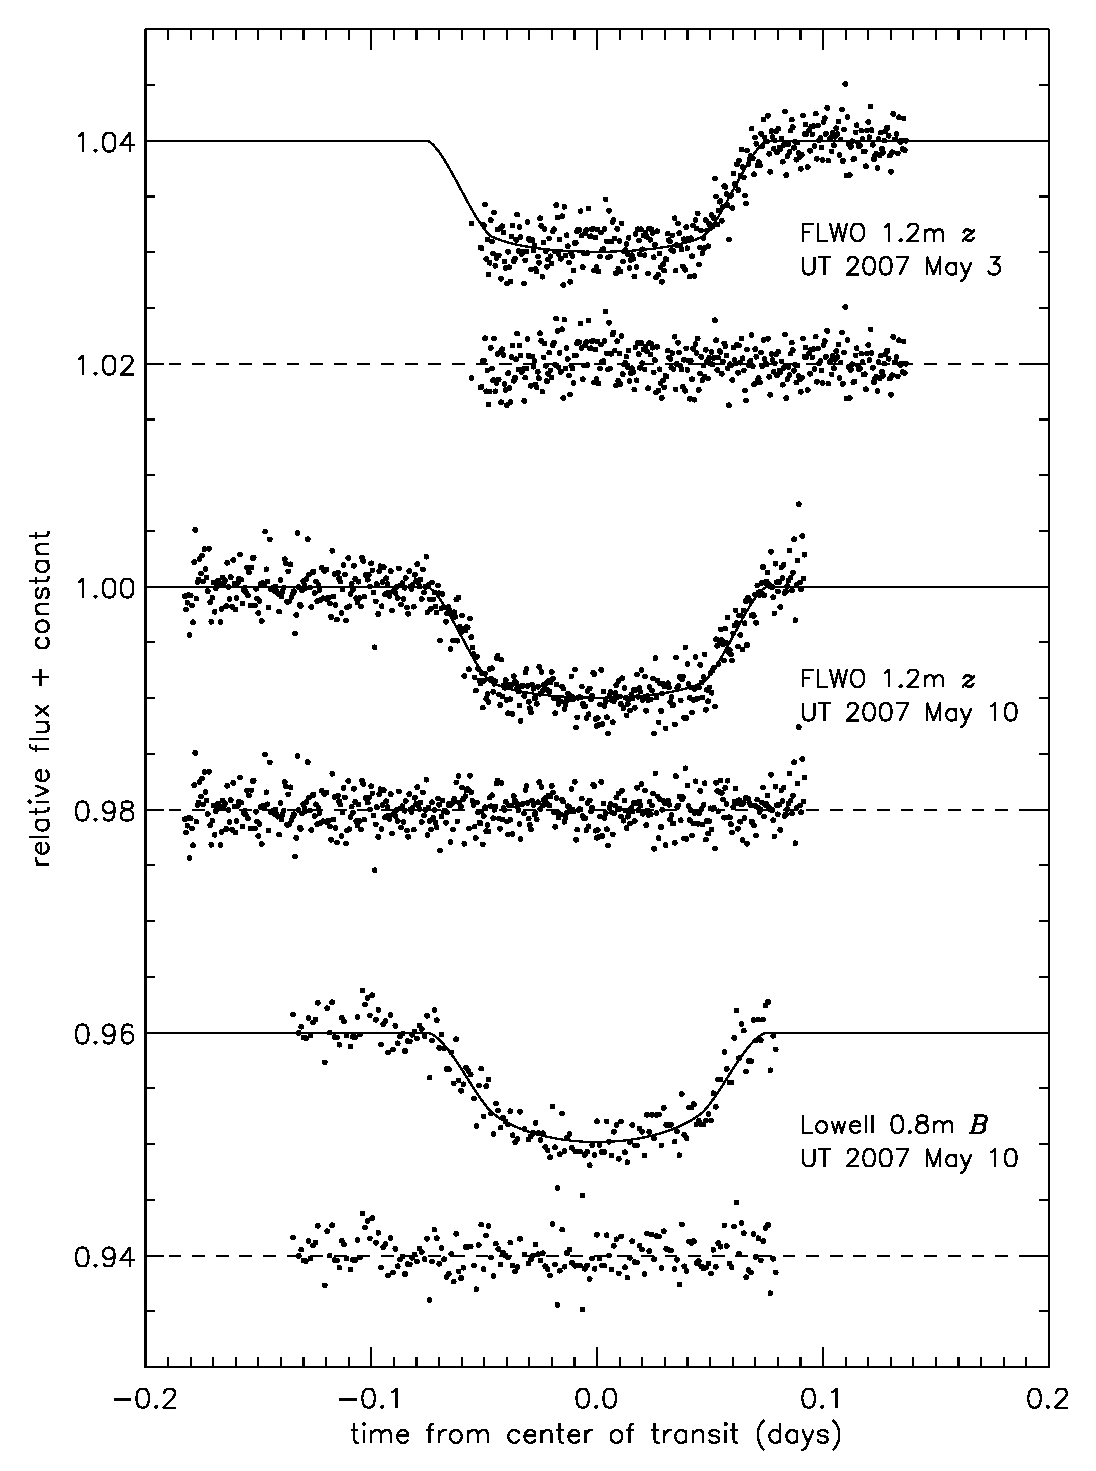
\includegraphics[width=0.95\textwidth]{A_TrES4_f1}
\caption[High-precision follow-up $z$-band and $B$-band photometry of \tresFour]{High-precision follow-up $z$-band and $B$-band photometry of \tresFour.
The plot shows the 
relative flux (including the color-dependent extinction correction) of the 
\tresFour\ system as a function of time relative to the center of transit, 
adopting the ephemeris in table~\ref{cha:tres4:sec:obs:tab:planet}. Each light curve is labeled with the telescope and date of observation. The residuals from the simultaneous 
fits (\textit{solid lines}) are shown below each light curve. 
\label{cha:tres4:sec:obs:fig:phot}}
\end{figure}

We carried out 
high-precision in-transit $z$-band photometry of \tresFour\ on UT 2007 May~3 and 
UT 2007 May~10 with KeplerCam \citep[see, e.g.,][]{Holman_Winn_Latham:apj:2006a} at the Fred~L.~Whipple Observatory (FLWO) 1.2-meter telescope, and $B$-band photometry on UT 2007 May~10 using NASACam at the Lowell Observatory 0.8-meter telescope. With 
KeplerCam we gathered 373 and 540 $z$-band 30-second exposures on UT 2007 May~3 and UT 2007 May~10, respectively.
With NASACam, we%observed an $18\arcmin \times 18\arcmin$ field around \tresFour\ and gathered 
\ obtained 192 60-second $B$-band exposures%
. For both data sets, we derived differential fluxes relative to an 
ensemble of local comparison stars. The%
\ photometry is shown in figure~\ref{cha:tres4:sec:obs:fig:phot}.

\begin{deluxetable}{lr}
\tablewidth{0pt}
\tablecaption{Radial-velocity measurements of \tresFour\ \label{cha:tres4:sec:obs:tab:rv}}
\tablehead{
\colhead{HJD} & \colhead{\ \ RV (\ms)}}
\startdata
2454187.07793  &  \phm{-}$ 97.5 \pm 11.8$ \\
2454188.11122  &  \phm{-}$ 58.9 \pm \phn 9.4$ \\
2454189.02631  &  $-76.5 \pm 11.6$ \\
2454189.14920  &  $-73.9 \pm 10.3$ \\
\enddata
\end{deluxetable}

We obtained high-precision RV measurements of \tresFour\ on UT 2007 March~27--29, 
using HIRES and its I$_2$ absorption cell \citep{Vogt_Allen_Bigelow:SPIE:1994a} on the Keck~I telescope. 
Our spectra have a nominal resolving power $\lambda/\Delta\lambda\simeq 55\,000$ and a typical signal-to-noise ratio $S/N\sim 120$~pixel$^{-1}$.
We used nine echelle orders in the wavelength range 3200--8800\,\AA\ to derive the velocities for \tresFour.
The four star-plus-I$_2$ spectra (plus one I$_2$-free 
template exposure) provide good coverage of the critical phases. As the 
ephemeris of the system is fixed, RV data are needed only to 
determine the amplitude and systemic velocity of the orbit. In these cases 
\citep[see][]{Konacki_Torres_Jha:nat:2003a} a few measurements are enough. 
We extracted and reduced all raw spectra using the MAKEE software 
written by T.~Barlow (
\citealp{Sozzetti_Torres_Latham:apj:2006a}
).
 The final RV values are 
listed in table~\ref{cha:tres4:sec:obs:tab:rv}. 
The typical precision of the radial velocities 
$\left \langle \sigma_{RV} \right \rangle \simeq 10 \, \ms$ is slightly 
degraded by the modest stellar rotation. 
The high-resolution, high $S/N$ Keck spectra were then used to rule out blend 
scenarios (see below), and they are presently 
being analyzed for improved characterization of the host star.

\begin{figure}
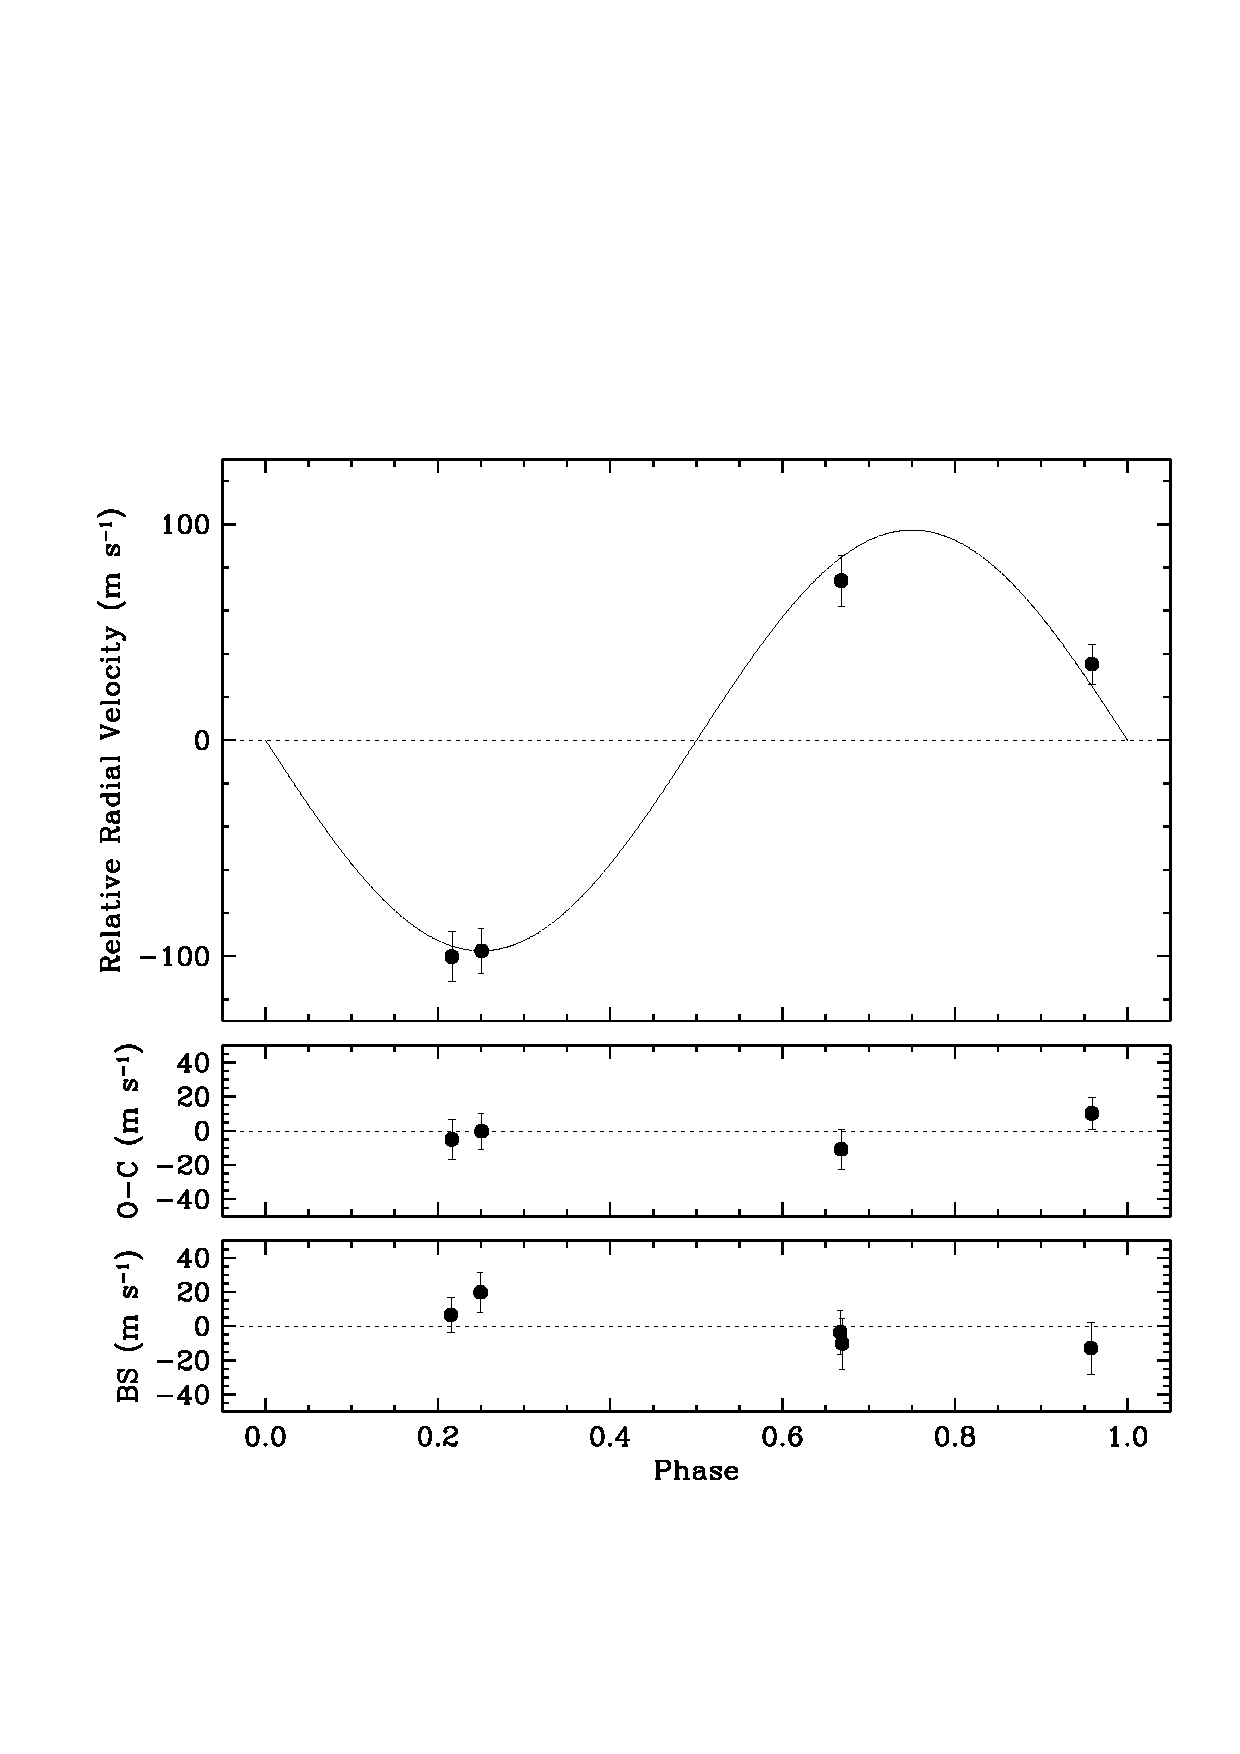
\includegraphics[width=0.95\textwidth]{A_TrES4_f2}
\caption[Keck/HIRES radial velocity observations of \tresFour]{({\em Top}) Radial velocity observations of \tresFour\ obtained with 
Keck/HIRES using the I$_2$ cell, shown relative to the center of mass and 
adopting the ephemeris in table~\ref{cha:tres4:sec:obs:tab:planet}. The best-fit orbit 
({\em solid line}) is overplotted. ({\em Middle}) Residuals from the best-fit 
model to the radial velocities. ({\em Bottom}) Bisector spans shifted to a 
median of zero, for each of the iodine exposures as well as for the template 
(which is shown as an additional point at phase 0.669). \label{cha:tres4:sec:obs:fig:rv}}
\end{figure}

We fit a Keplerian orbit to these data assuming zero eccentricity as a good 
first approximation, as expected from theoretical arguments for a period as 
short as 3.55~days. The period and epoch of transit were held fixed. The rms of 
this fit is 11~\ms, which is similar to the internal errors of the velocities. 
The parameters of this orbital solution are listed in table~\ref{cha:tres4:sec:obs:tab:planet}. We 
find \mbox{$M_{\rm p} \sin i = 0.731 \pm 0.057~[(M_{\star} + M_{\rm p})/M_{\sun}]^{2/3}$~$M_{\rm Jup}$}. 
The orbit is displayed in figure~\ref{cha:tres4:sec:obs:fig:rv} ({\it top panel}) along with the 
observations, and residuals are shown in the {\it middle panel}.

We investigated the possibility that the RV variations we measured are the 
result of distortions in the line profiles caused by contamination from an 
unresolved eclipsing binary \citep{Santos_Mayor_Naef:aa:2002a, Torres_Konacki_Sasselov:apj:2005a}, instead of being caused by a planetary companion. We cross-correlated 
each Keck spectrum against a synthetic template matching the properties of the 
star, and averaged the correlation functions over all orders blueward of the 
region affected by the I$_2$ lines. From this representation of the average 
spectral line profile we computed the mean bisectors, and as a measure of the
line asymmetry we calculated the ``bisector spans" as the velocity difference 
between points selected near the top and bottom of the mean bisectors 
\citep{Torres_Konacki_Sasselov:apj:2005a}. If the RV variations were the result of a blend with an eclipsing 
binary, we would expect the line bisectors to vary in phase with the 
photometric period with an amplitude similar to that of the velocities 
\citep{Queloz_Henry_Sivan:aa:2001a, Mandushev_Torres_Latham:apj:2005a}. Instead, we detect no variation in excess of the 
measurement uncertainties (see figure~\ref{cha:tres4:sec:obs:fig:rv}, {\it bottom panel}), and we conclude 
that the RV variations are real and that the star is orbited by a Jovian 
planet.

\section{Properties of \tresFour\ and Discussion}
\label{cha:tres4:sec:dis}


We analyzed the two $z$-band and one $B$-band photometric time series using the 
analytic light curves of \citet{Mandel_Agol:apjl:2002a}. We assumed a circular orbit and a 
quadratic stellar limb-darkening law, fixing the coefficients at the 
color-dependent values tabulated in \citet{Claret:aa:2000a, Claret:aa:2004a} for the 
spectroscopically estimated $T_{\rm eff}$ and $\log g$, and assuming solar 
metallicity. We first estimated the time of center of transit $T_c$ by fitting 
a model light curve to the $z$ data gathered on UT 2007 May~10. We then determined the orbital period $P$ by combining these 
data with the TrES discovery data (which affords a baseline of 1.0\,yrs)
varying the trial values of $P$
. We then fixed the values of $T_c$ and $P$ 
(stated in table~\ref{cha:tres4:sec:obs:tab:planet}) in the subsequent analysis.

Our model has six free parameters: the planet radius $R_{\rm p}$, the stellar 
radius $R_{\star}$, the orbital inclination $i$, and the color-dependent extinction for each of the three photometric datasets, 
$k_{z1}$, $k_{z2}$, and $k_B$. We assume that the observed flux is proportional 
to $e^{-km}$, where $m$ denotes the air mass. The values of $R_{\rm p}$ and 
$R_{\star}$ as constrained by the light curves alone are covariant with 
$M_{\star}$. In our analysis, we first estimated the quantity $a / R_{\star}$ which 
is independent of the assumed value of $M_{\star}$, and then used this estimate 
to constrain the value of $M_{\star}$ from stellar isochrones 
\citep{Sozzetti_Torres_Charbonneau:apj:2007a, Holman_Winn_Latham:apj:2007a}. We then fixed $M_{\star} = 1.22$~$M_{\sun}$, and 
estimated the systematic error in the radii using the scaling 
relations $R_{\rm p} \propto R_{\star} \propto M_{\star}^{1/3}$ (see footnote to 
table~\ref{cha:tres4:sec:obs:tab:host_star}).

We found first the values of $R_{\rm p}$, $R_{\star}$, $i$, $k_{z1}$, $k_{z2}$, 
and $k_B$ that minimized the ${\chi}^{2}$ using the AMOEBA algorithm 
\citep{Press_Teukolsky_Vetterling:1992a}. This model is shown as the solid curves in figure~\ref{cha:tres4:sec:obs:fig:phot}. 
We then conducted a Markov Chain Monte Carlo analysis similar to that described 
in \citet{Holman_Winn_Latham:apj:2006a}, \citet{Charbonneau_Winn_Everett:apj:2007a}, and \citet{Winn_Holman_Roussanova:apj:2007a}. 
We created two MCMC chains 
with 400,000 points each, one starting from the best-fit values and one 
starting from a random perturbation to those values. We 
then rejected the first 23\% of the points to minimize the impact of 
the initial conditions and found the results from the two chains to be 
indistinguishable. We examined the histograms of the six parameters, as well as 
the histograms for several combinations of parameters relevant to anticipated 
follow-up studies. We assigned the optimal value to the median, and the 
1-$\sigma$ errors to the symmetric range about the median than encompassed 
68.3\% of the values. We list these estimates in table~\ref{cha:tres4:sec:obs:tab:planet}. 

\tresFour\ has the largest radius and the lowest density of all exoplanets whose 
mass and radius are known, and as such presents new challenges for the theory 
of irradiated gas giants. \citet{Burrows_Hubeny_Budaj:apj:2007a} suggested that increased planetary atmospheric opacities and the inclusion of a transit radius correction 
(\citealp{Baraffe_Chabrier_Barman:aa:2003a}; \citealp*{Burrows_Sudarsky_Hubbard:apj:2003a}) can explain the radii of all large planets. It appears, 
however, that \tresFour's radius is still too large for its mass, age and 
insolation. In terms of mass and distance to the host star \tresFour\ is similar 
to \hdTZN, but has nearly 30\% larger radius ($R_{\rm p} = 1.67\,\rjup$ versus $R_{\rm p} = 1.32\,\rjup$). Because of the higher host star luminosity \tresFour\ receives about twice the stellar flux, but it is unlikely that the radius difference can be explained solely by the higher stellar 
irradiation. For example, \hatponeb, which has about the same radius as 
\hdTZN\ and is the only other planet with $\rho < 0.3$~${\rm g \: cm^{-3}}$, 
receives only 60\% of the flux that \hdTZN\ does. None of the recent models 
of hot Jupiters (\citealp*[e.g.,][]{Fortney_Marley_Barnes:apj:2007a}; \citealp{Burrows_Hubeny_Budaj:apj:2007a}) can predict a radius as 
large as that of \tresFour\ at its orbital separation for the estimated age and 
for any mass, even when higher atmospheric opacities are considered and 
allowance for the transit radius correction is made.

The properties of \tresFour\ and its host star allow for many interesting follow-up 
studies, some of which are already underway. The large radius of \tresFour\ in the 
visual suggests that it may have an extended outer atmosphere, similar to that 
detected around \hdTZN\ in Lyman~$\alpha$ by \citet{Vidal-Madjar_Lecavelier-des-Etangs_Desert:nat:2003a}. If such an 
extended envelope is caused by mass loss through the planet's Roche lobe 
boundary, \tresFour\ may have an even bigger envelope because of its smaller 
Roche limit: $R_{\rm Roche} \approx 3.5$~$R_{\rm p}$ versus 
$R_{\rm Roche} \approx 4.4$~$R_{\rm p}$ for HD209458b \citep{Erkaev_Lammer_Kulikov:preprint:2007a}. 
Moreover, \tresFour\ might be in a strong hydrodynamic ``blow-off" regime where the 
outer atmospheric layers are detached from the planet's gravitational field and 
escape in a comet-like tail \citep{Vidal-Madjar_Lecavelier-des-Etangs_Desert:nat:2003a, Lecavelier-des-Etangs_Vidal-Madjar_McConnell:aa:2004a}.

The relatively fast rotation ($v \sin i = 9.5 \, \kms$) and brightness of the 
\tresFour's host star, as well as the planet's size, are favorable for measuring 
the Rossiter-McLaughlin effect (RME; \citealp[see, e.g.,][]{Gaudi_Winn:apj:2007a}). Of 
particular interest is the angle between the star's spin axis and the planet's 
orbital plane, as it can provide information about the possible mechanisms of 
the planet migration and interaction with the disk. The semi-amplitude of the 
RME is proportional to $v \sin i$ and to $(R_{\rm p} / R_{\star})^2$ and we 
estimate that for \tresFour\ the RME can reach about $90~\ms$, or roughly equal to 
the semi-amplitude of its orbital velocity. 


